\documentclass[10pt]{article}

% Lines beginning with the percent sign are comments
% This file has been commented to help you understand more about LaTeX

% DO NOT EDIT THE LINES BETWEEN THE TWO LONG HORIZONTAL LINES

%---------------------------------------------------------------------------------------------------------

% Packages add extra functionality.
\usepackage{times,graphicx,epstopdf,fancyhdr,amsfonts,amsthm,amsmath,algorithm,algorithmic,xspace,hyperref}
\usepackage[left=1in,top=1in,right=1in,bottom=1in]{geometry}
\usepackage{sect sty}	%For centering section headings
\usepackage{enumerate}	%Allows more labeling options for enumerate environments 
\usepackage{epsfig}
\usepackage[space]{grffile}
\usepackage{booktabs}
\usepackage{forest}
\usepackage{paracol}

\usepackage{tikz}
\usetikzlibrary{arrows.meta,positioning}

% This will set LaTeX to look for figures in the same directory as the .tex file
\graphicspath{.} % The dot means current directory.

\pagestyle{fancy}

\lhead{Final Project}
\rhead{\today}
\lfoot{CSCI 334: Principles of Programming Languages}
\cfoot{\thepage}
\rfoot{Fall 2023}

% Some commands for changing header and footer format
\renewcommand{\headrulewidth}{0.4pt}
\renewcommand{\headwidth}{\textwidth}
\renewcommand{\footrulewidth}{0.4pt}

% These let you use common environments
\newtheorem{claim}{Claim}
\newtheorem{definition}{Definition}
\newtheorem{theorem}{Theorem}
\newtheorem{lemma}{Lemma}
\newtheorem{observation}{Observation}
\newtheorem{question}{Question}

\setlength{\parindent}{0cm}


%---------------------------------------------------------------------------------------------------------

% DON'T CHANGE ANYTHING ABOVE HERE

% Edit below as instructed

\begin{document}
  
\section*{\textit{Pül}: Project Proposal}

Jacob Cohen, Kevin Pepin\\
Video link: \url{https://youtu.be/PTQFD-OmYUk}

\subsection{Introduction}

This scheduling language is motivated by a common ride-share problem that Williams students face. Amongst students groups, friend groups, and even campus-wide, it is common for those with cars at Williams to offer rides to those that don't have one. On the track and field team, someone might offer a ride to NYC at 2pm next Friday or to Boston the Tuesday before Thanksgiving. On the other side, someone might request a ride to the Albany airport next Saturday to catch their flight or to the Pittsfield Target to get some room supplies. With only a few offers and requests, the requestors can just check to see if there's an offer that fits their needs. However, during school breaks, when the offer/request list is massive, finding a valid matching of offers and requests can be quite tedious. A language composed of standardized offer and request entries could allow programmers to model any rapidly evolving offer/request list given any number of constraints.\\
\\
By making this a programming language, it can handle any sized input program that evaluates with consistent results. A program can consist of any number of offers/requests. It has the flexibility to find carpools for a small number of people. As you can see in the four example programs below, this is fairly trivial to also do by hand. But, the same language can find carpools across the entire Williams campus of 2,000 people. Imagine a sample program like the ones below but with hundreds of lines. Trying to keep track of such a large amount of requests and offers by hand is no longer a viable option.\\
\\
Since a program is just a collection of request and offers, if someone decides they won't be driving and revokes their offer, then finding a new carpool setup is just a matter of removing a line of the program and re-evaluating it. Similarly, changing a request or offer's data is merely a change in the program. Regardless of the size of your program, if you need to make changes to the input, recomputing the result simply involves re-evaluating the new program.\\
\\
As a programming language, it can be expanded to accept as many formats and include as many constraints as we'd like. If you wanted to accept some other date format, you'd only need to add a new parser for that date format. If you wanted to allow for anonymous offers you could edit the parser to look for zero or more names. Since only the format of the input program changes, none of the interpretation and evaluation breaks, as long as the new parser follows the existing ADT's. Likewise, you may want to add new input fields. Maybe you want to consider the limited baggage space in vehicles? Or you are willing to pay money for your request? Or you are only willing to accept above a certain amount for your offer? Regardless of the extension, this programming language can evolve to include these restrictions. We can add any additional features to our requests/offers in our programming language as long as we parse them, pass them to the evaluator, and modify the evaluator to actually consider them.

\newpage
\subsection{Design Principles}

The backbone of this language is that one can represent the carpool match-making space via two main types: offers and requests. An offer embodies all crucial information pertaining to someone who has space to take more people in their vehicle. Likewise, a request represents someone who is searching for a seat to somewhere. Each is a combining form containing several primitive types (or near primitive types) that make each offer or request unique.\\
\\
A program in this language is some example scenario of offers and requests which looks like a list of them. This design choice allows individual offers/requests to be easily modified in a program and allows for a program to be infinitely long. This language syntax is intuitive because a program resembles the group chat that motivated the programming language where we can imagine multiple people would have communicated unstandardized offers and requests for rides. For example, one could translate the chat below into the program below it:

\medskip
\textbf{An Imaginary Group Chat}\\
\textit{Cooper}: Can anyone give me a ride to Bennington tomorrow?\\
\textit{Jacob}: I'm heading home to NYC tonight if anyone needs a ride.\\
\textit{Jack}: I'm headed to Boston after practice today.\\
\textit{Oscar}: Could I get a ride to the airport tomorrow before my 6am flight?

\medskip
\textbf{Represented as a Program}\\
\verb|Request: Cooper to Bennington at 12 AM on 12/2/2023 to 11 PM on 12/3/2023|\\
\verb|Offer: Jacob to NYC at 5 PM on 12/1/2023 to 8 PM on 12/1/2023 with 3 seats|\\
\verb|Offer: Jack to Boston at 6 PM on 12/1/2023 with 4 seats|\\
\verb|Request: Oscar to Albany at 4 AM on 12/2/2023|

\medskip
Notice that, accounting for interpreting colloquial terms like ``tonight" and ``after practice," the program is visually similar to the group chat messages that inspired its creation. Thus, rather than hashing out the carpools with a bunch of texts in the group chat, one could evaluate the program above.

\newpage
\subsection{Examples}

You'll find multiple example programs in $code/Project/ExamplePrograms/$. Several key ones are listed here with example outputs. Additional ones are included at the path above and all may be run with\\
\verb|dotnet run <path to example program>| at the $Project$ level.

\begin{enumerate}
    \item[1)] A super basic program where the output matches the only offer and request.
\begin{verbatim}
Offer: Jacob to NYC at 2 PM on 11/5/2023 to 4 PM on 11/6/2023 with 3 seats 
Request: Oscar to NYC at 3 PM on 11/5/2023
\end{verbatim}
The expected output is \scriptsize
\begin{verbatim}
MATCHED REQUESTS:
    Oscar to NYC at 3 PM on 11/5/2023 -> Jacob to NYC at 2 PM on 11/5/2023 to 4 PM on 11/6/2023
\end{verbatim} \normalsize
Evaluated programs return all the requests in the program organized into a ``MATCHED REQUESTS" section and an ``UNMATCHED REQUESTS" section (doesn't appear here since there aren't any, see later programs for ones with unmatched requests). Each request is followed by the offer (minus its seat info) that will fulfil it. The returned output is the maximum number of requests that can be fulfilled by the program's offers subject to the constraints in the program.

    \item[2)]  A more complex program where the output matches multiple offers and requests.
\begin{verbatim}
Offer: Jacob to NYC at 2 PM on 11/5/2023 to 4 PM on 11/6/2023 with 3 seats 
Offer: Jack to Boston at 12 PM on 11/26/2023 with 1 seat
Request: Cooper to Boston at 12 PM on 11/26/2023
Request: Oscar to NYC at 9 AM on 11/5/2023 to 5 PM on 11/5/2023
\end{verbatim}
    The expected output is \scriptsize
\begin{verbatim}
MATCHED REQUESTS:
    Cooper to Boston at 12 PM on 11/26/2023 -> Jack to Boston at 12 PM on 11/26/2023
    Oscar to NYC at 9 AM on 11/5/2023 to 5 PM on 11/5/2023 -> Jacob to NYC at 2 PM on 11/5/2023 to 4 PM on 11/6/2023
\end{verbatim} \normalsize

    \item[3)] This one builds on the last by demonstrating the list of locations feature as well as showing what happens with unmatched offers and requests.
\begin{verbatim}
Request: Cooper to Springfield, Pittsfield, Boston at 12 PM on 11/26/2023
Request: Oscar to NYC, Westchester at 3 PM on 11/5/2023
Request: Camryn to Calgary at 9 AM on 11/5/2023
Offer: Jacob to NYC at 2 PM on 11/5/2023 to 4 PM on 11/5/2023 with 3 seats
Offer: Jack to Boston at 12 PM on 11/26/2023 with 1 seat
Offer: Andrew to Annaheim at 12 PM on 11/26/2023 with 1 seat
\end{verbatim}
    The expected output is \scriptsize
\begin{verbatim}
MATCHED REQUESTS:
    Cooper to Springfield, Pittsfield, Boston at 12 PM on 11/26/2023 -> Jack to Boston at 12 PM on 11/26/2023
    Oscar to NYC, Westchester at 3 PM on 11/5/2023 -> Jacob to NYC at 2 PM on 11/5/2023 to 4 PM on 11/5/2023

UNMATCHED REQUESTS:
    Camryn to Calgary at 9 AM on 11/5/2023
\end{verbatim} \normalsize
This is the first example where we see unmatched and matched requests. Notice that the unmatched requests are listed in their own section with no offer following them. We do not print unmatched offers (AKA Andrew in this example) since the output is intended to help requestors find their ride, so it does not matter to Andrew that no one is riding in his car.

    \item[4)] This one is much longer and incorporates all of the languages features. One may have noticed that manually computing the answers to the above examples isn't that difficult. The power of this programming language is that in can handle longer programs like the one below which become exponentially more challenging to compute by hand.
\begin{verbatim}
Offer: Abe to Arlington at 2 PM on 1/5/2023 to 6 PM on 1/5/2023 with 2 seat
Request: Bob to Boston at 5 PM on 1/3/2023
Offer: Cam to Chicago at 2 AM on 5/22/2023 to 10 AM on 5/23/2023 with 4 seats
Request: Dan to Denver at 9 PM on 11/27/2023
Request: Echo to Chicago at 10 PM on 5/22/2023
Request: Fay to Chicago at 10 PM on 5/22/2023
Request: Gabe to Arlington, Chicago at 5 PM on 1/1/2023 to 5 PM on 5/22/2023
Request: Hay to Arlington at 1 AM on 1/1/2023 to 11 PM on 1/9/2023
\end{verbatim}
The expected output is \scriptsize
\begin{verbatim}
MATCHED REQUESTS:
    Echo to Chicago at 10 PM on 5/22/2023 -> Cam to Chicago at 2 AM on 5/22/2023 to 10 AM on 5/23/2023
    Fay to Chicago at 10 PM on 5/22/2023 -> Cam to Chicago at 2 AM on 5/22/2023 to 10 AM on 5/23/2023
    Gabe to Arlington, Chicago at 5 PM on 1/1/2023 to 5 PM on 5/22/2023 -> Abe to Arlington at 2 PM on 1/5/2023 to 6 PM on 1/5/2023
    Hay to Arlington at 1 AM on 1/1/2023 to 11 PM on 1/9/2023 -> Abe to Arlington at 2 PM on 1/5/2023 to 6 PM on 1/5/2023

UNMATCHED REQUESTS:
    Bob to Boston at 5 PM on 1/3/2023
    Dan to Denver at 9 PM on 11/27/2023
\end{verbatim} \normalsize
\end{enumerate}

\newpage
\subsection{Language Concepts}
% A walkthrough of the BNF

A program in our language represents a series of events to help organize rides amongst students. A brand new program with nothing in it represents an empty $inputSchedule$. An $inputSchedule$ can contain two kinds of events: a $request$ or an $offer$. In order to write a $request$, the user must write a line in the format below: 

\begin{center}Request: \textit{name} to \textit{locationList} at \textit{timeRange}.\end{center}

The string entered in the place of \textit{name} will be the name by which the request is identified. \textit{locationList} can either contain a single location or a list of locations which the person submitting this request is willing to be dropped off at. \textit{timeRange} is the time and date (or times and dates) at which the person requesting the ride would like to leave on their ride to any of their given locations. An example of a $timeRange$ would be: 

\begin{center} at 2 PM on 1/5/2023 to 6 PM on 1/5/2023 \end{center}

If the above $timeRange$ were included in a request, it would signify that the person requesting the ride would be willing to be picked up from 2 PM to 6 PM on January 5th, 2023.\\\\
In addition to a request, the other object accepted in the $inputSchedule$ is an $offer$ object. The $offer$ constructor follows the following format:

\begin{center}Offer: \textit{name} to \textit{locations} at \textit{timeRange} with \textit{seatCount} \textit{seatString}.\end{center}

Similar to the request constructor, \textit{name} is the string by which the offer is identified, and \textit{location} is the place the offering driver is going. A $timeRange$ in the offer constructor represents the times when a driver is offering to depart for a location. \\\\
The primary distinction between the request and offer constructor are the \textit{seatCount} and \textit{seatString} parameters. These two parameters are present in the offer constructor only in order to provide the number of people the person offering a ride is willing to take, with $seatString$ being ``seat" or ``seats" depending on value of $seatCount$. An offer where the driver is only willing to take one other person would end with the following combination of $seatCount$ and $seatString$:

\begin{center} ...with 1 seat.\end{center}

While an offer to drive more than one person would contain the number of available seats and the word ``seats"


\begin{center} ...with 3 seats.\end{center}

We then use these requests and offers to organize carpools. While there is no guarantee that all requests will be satisfied, we can guarantee that the maximum possible number of requests will be satisfied in the output given the program's constraints. The outputs will be organized by those requests which were satisfied, and those which were not. First there will be a line which reads ``MATCHED REQUESTS:", below which all of the requests in the given program which are satisfied by the offers listed in the program. Below those requests, there is a line which reads ``UNMATCHED REQUESTS". Beneath that line, there will be all of the requests which are unable to be serviced given the offers of the input program. 

\newpage
\subsection{Syntax}

A complete BNF for programs written in our language. Anywhere there is white space, one or more white space characters are allowed.

\begin{verbatim}
<inputSchedule>    ::= <event> <inputSchedule>
                    |  <event>
<event>            ::= <offer>
                    |  <request>
<offer>            ::= Offer: <name> to <location> at <timeRange> with <seatNum> <seatStr>
<request>          ::= Request: <name> to <locationList> at <timeRange>
<timeRange>        ::= <time>
                    |  <time> to <time>
<time>             ::= <hour> on <date>
<locationList>     ::= <location>
                    |  <location>, <locationList>
<name>             ::= <letter>+
<location>         ::= <letter>+
<hour>             ::= <hourNum> <hourStr>
<hourNum>          ::= Z \in [1,12]
<hourStr>          ::= AM | PM
<date>             ::= <monthNum>/<day>/<year>
<monthNum>         ::= Z \in [1,12]
<seatNum>          ::= <digit>+
<seatStr>          ::= seats | seat
<day>              ::= Z \in [1,31]
<year>             ::= 2023
<digit>            ::= 0 | 1 | 2 | 3 | 4 | 5 | 6 | 7 | 8 | 9
<letter>           ::= \alpha \in {a...z}
                    |  \alpha \in {A...Z}
\end{verbatim}
%<hour>             ::= 0 | 1 | 2 | 3 | 4 | 5 | 6 | 7 | 8 | 9 | 10 | 11 | 12 | 13 |
%                       14 | 15 | 16 | 17 | 18 | 19 | 20 | 21 | 22 | 23 | 24
%<month>            ::= 0 | 1 | 2 | 3 | 4 | 5 | 6 | 7 | 8 | 9 | 10 | 11 | 12
%<day>              ::= 0 | 1 | 2 | 3 | 4 | 5 | 6 | 7 | 8 | 9 | 10 | 11 | 12 | 13 |
%                       14 | 15 | 16 | 17 | 18 | 19 | 20 | 21 | 22 | 23 | 24 | 25 |
%                       26 | 27 | 28 | 29 | 30 | 31

\newpage
\subsection{Semantics}
\subsubsection{BNF Element Semantics and ADT's}
\begin{itemize}
    \item $letter$ is a primitive. We represent letters using the F\# \verb|char| data type. 
    \item $digit$ is another primitive in our language. We represent a digit by using the F\# \verb|int| data type to store the values from 0 - 9. 
    \item $year$ is a primitive in our language used in the date type. $year$ can only be one value, the \verb|int| 2023. 
    \item $day$ uses the F\# \verb|int| type to represent the day a request or offer is being made to.  $day$ can only be an integer  between $1$ and $31$ inclusive, as any value within that range should be a valid day of a month.
    \item $seatStr$ is an F\# \verb|String| which can either be ``seat" or ``seats" depending on the value of $seatNum$.
    \item $seatNum$ is an F\# \verb|int| made of $1$ or more digits which represents the number of seats available in an offer.
    \item $monthNum$ is an F\# \verb|int| representation of the month for a specific $date$ that a request/offer is valid for.
    \item $date$ represents the full date of the offer/request by taking the previously mentioned $monthNum$, $day$, and $year$. It is not specifically stored by any ADT in our parser but is stored later on in $time$ with other types. 
    \item $hourStr$ is an F\# \verb|String| which can only either be ``AM" or ``PM", and is used in the $hour$ constructor to indicate the time at which the offer/request is relevant to. 
    \item $hourNum$ is an F\# \verb|int| between $1$ and $12$ inclusive which is used in the $hour$ constructor to indicate the time at which the offer/request is relevant to.
    \item $hour$ represents the hour at which at an offer/request is valid by combining an $hourNum$ and an $hourStr$. 
    \item $location$ is an F\# \verb|String| which takes one or more $letter$'s to create the name of where an offer/request goes. 
    \item $locationList$ is an F\# \verb|String List| which contains one or more $location$ types. It represents a singular location or multiple locations, which accounts for the scenario during which someone is willing to be dropped off at different locations. 
    \item $name$ is an F\# \verb|String| which takes one or more $letter$'s to create the name of the individual either requesting a ride or offering a ride to someone else. 
    \item $time$ is an F\# \verb|DateTime| type which combines the previously mentioned $hour$ object as well as a $date$ object to give the full time at which an individual is willing to be dropped off/ pick someone else up.
    \item $timeRange$ is an ADT defined below which takes either a singular time object, or can take two time objects in the case that someone is willing to be picked up between two times, or is willing to pick others up between two times. Its type signature is $DateTime\to DateTime\to TimeRange$.
    \begin{verbatim}
type TimeRange = {startTime: DateTime; endTime: DateTime}\end{verbatim}
    \item $request$ is a constructor which takes a $name$, $locationList$, and $timeRange$ to create a record of a request for a ride being made. It is a constructor for the $event$ ADT defined below. Its type signature is $name\to locationList \to timeRange\to Event$.
    \item $offer$ is a constructor which takes a $name$, $location$, $timeRange$, $seatNum$, and $seatStr$ in order to create record of an offer being made. It is a constructor for the $event$ ADT defined below. Its type signature is $name\to location \to timeRange\to seatNum\to Event$.
    \item an $event$ is the main ADT of the entire program. It can either be constructed via an $offer$ or a $request$. Its ADT definition is below:
    \begin{verbatim}
type Event =
| Offer of string * string List * TimeRange * int
| Request of string * string List * TimeRange\end{verbatim}
    \item $inputSchedule$ is an \verb|Event List| and is the backbone of the programming language. An input schedule can either be one $event$, or an $event$ and an $inputSchedule$, which is to say, multiple events. Its ADT is defined as follows:
    \begin{verbatim}
type InputSchedule = Event list\end{verbatim}
\end{itemize}

\newpage
\subsubsection{AST For Example Program One}
We can make an AST for the first example program which is repeated here for reference. Note that this AST uses $()$ in place of $<>$ to save space width wise.
\begin{verbatim}
Offer: Jacob to NYC at 2 PM on 11/5/2023 to 4 PM on 11/6/2023 with 3 seats 
Request: Oscar to NYC at 3 PM on 11/5/2023
\end{verbatim}
    \scalebox{0.75}{
    \rotatebox{0}{
    \begin{forest}
      [(inputSchedule)
        [(event)+
            [(offer)
                [{(name, location, timeRange, seatNum, seatStr)}
                    [(name)
                        [Jacob]
                    ]
                    [(location)
                        [NYC]
                    ]
                    [(timeRange)
                        [{(time, time)}
                            [{(hour, date)}
                                [(hourNum)(hourStr)
                                    [2]
                                    [PM]
                                ]
                                [{(monthNum, day, year)}
                                    [11]
                                    [5]
                                    [2023]
                                ]
                            ]
                            [{(hour, date)}
                                [(hourNum)(hourStr)
                                    [4]
                                    [PM]
                                ]
                                [{(monthNum, day, year)}
                                    [11]
                                    [6]
                                    [2023]
                                ]
                            ]
                        ]
                    ]
                    [(seatNum)
                        [(digit)+
                            [3]
                        ]
                    ]
                    [(seatStr)
                        [seats]
                    ]
                ]
            ]
            [(request)
                [{(name, location, timeRange)}
                    [(name)
                        [Oscar]
                    ]
                    [(locationList)
                        [(location)
                            [NYC]
                        ]
                    ]
                    [(timeRange)
                        [{(time)}
                            [{(hour, date)}
                                [(hourNum)(hourStr)
                                    [3]
                                    [PM]
                                ]
                                [{(monthNum, day, year)}
                                    [11]
                                    [5]
                                    [2023]
                                ]
                            ]
                        ]
                    ]
                ]
            ]
        ]
      ]
    \end{forest}
    }
    }

\newpage
\subsubsection{AST For Example Program Two}
For the second program we have
      \begin{verbatim}
Offer: Jacob to NYC at 2 PM on 11/5/2023 to 4 PM on 11/6/2023 with 3 seats
Offer: Jack to Boston at 12 PM on 11/26/2023 with 1 seat
Request: Cooper to Boston at 12 PM on 11/26/2023
Request: Oscar to NYC at 9 AM on 11/5/2023 to 5 PM on 11/5/2023
\end{verbatim}
\scalebox{0.4}{
    \rotatebox{90}{
    \begin{forest}
      [(inputSchedule)
        [(event)+
            [(offer)
                [{(name, location, timeRange, seatNum, seatStr)}
                    [(name)
                        [Jacob]
                    ]
                    [(location)
                        [NYC]
                    ]
                    [(timeRange)
                        [{(time, time)}
                            [{(hour, date)}
                                [(hourNum)(hourStr)
                                    [2]
                                    [PM]
                                ]
                                [{(monthNum, day, year)}
                                    [11]
                                    [5]
                                    [2023]
                                ]
                            ]
                            [{(hour, date)}
                                [(hourNum)(hourStr)
                                    [4]
                                    [PM]
                                ]
                                [{(monthNum, day, year)}
                                    [11]
                                    [6]
                                    [2023]
                                ]
                            ]
                        ]
                    ]
                    [(seatNum)
                        [(digit)+
                            [3]
                        ]
                    ]
                    [(seatStr)
                        [seats]
                    ]
                ]
            ]
            [(offer)
                [{(name, location, timeRange, seatNum, seatStr)}
                    [(name)
                        [Jack]
                    ]
                    [(location)
                        [Boston]
                    ]
                    [(timeRange)
                        [{(time, time)}
                            [{(hour, date)}
                                [(hourNum)(hourStr)
                                    [12]
                                    [PM]
                                ]
                                [{(monthNum, day, year)}
                                    [11]
                                    [26]
                                    [2023]
                                ]
                            ]
                        ]
                    ]
                    [(seatNum)
                        [(digit)+
                            [1]
                        ]
                    ]
                    [(seatStr)
                        [seat]
                    ]
                ]
            ]
            [(request)
                [{(name, location, timeRange)}
                    [(name)
                        [Cooper]
                    ]
                    [(locationList)
                        [(location)
                            [Boston]
                        ]
                    ]
                    [(timeRange)
                        [{(time)}
                            [{(hour, date)}
                                [(hourNum)(hourStr)
                                    [12]
                                    [PM]
                                ]
                                [{(monthNum, day, year)}
                                    [11]
                                    [26]
                                    [2023]
                                ]
                            ]
                        ]
                    ]
                ]
            ]
            [(request)
                [{(name, location, timeRange)}
                    [(name)
                        [Oscar]
                    ]
                    [(locationList)
                        [(location)
                            [NYC]
                        ]
                    ]
                    [(timeRange)
                        [{(time)}
                            [{(hour, date)}
                                [(hourNum)(hourStr)
                                    [9]
                                    [AM]
                                ]
                                [{(monthNum, day, year)}
                                    [11]
                                    [5]
                                    [2023]
                                ]
                            ]
                            [{(hour, date)}
                                [(hourNum)(hourStr)
                                    [5]
                                    [PM]
                                ]
                                [{(monthNum, day, year)}
                                    [11]
                                    [5]
                                    [2023]
                                ]
                            ]
                        ]
                    ]
                ]
            ]
        ]
      ]
    \end{forest}
    }
    }

\newpage
\subsubsection{Evaluation For Example Program Four}
Let's consider the evaluation process for the fourth program reprinted here for convenience.
    \begin{verbatim}
Offer: Abe to Arlington at 2 PM on 1/5/2023 to 6 PM on 1/5/2023 with 2 seat
Request: Bob to Boston at 5 PM on 1/3/2023
Offer: Cam to Chicago at 2 AM on 5/22/2023 to 10 AM on 5/23/2023 with 4 seats
Request: Dan to Denver at 9 PM on 11/27/2023
Request: Echo to Chicago at 10 PM on 5/22/2023
Request: Fay to Chicago at 10 PM on 5/22/2023
Request: Gabe to Arlington, Chicago at 5 PM on 1/1/2023 to 5 PM on 5/22/2023
Request: Hay to Arlington at 1 AM on 1/1/2023 to 11 PM on 1/9/2023
\end{verbatim}
    The parser will convert this program into an $inputSchedule$ which is an \verb|Event List|. The $inputSchedule$ passed to the evaluator would look like
    \begin{verbatim}
thisInputScheule: Event List = [Offer(Abe,...); Request(Bob,...); Offer(Cam,...);...]
    \end{verbatim}
    The evaluator then takes these \verb|Event| types and constructs a flow network with them as follows:
    \begin{enumerate}
        \item Add a source node $s$ and sink node $t$
        \item Add \verb|Offer| nodes and \verb|Request| nodes
        \item Add an edge from the source $s$ to each offer with capacity of the offer's $seatNum$
        \item Add an edge with capacity $1$ from each offer to request if the offer satisfies the request
        \item Add an edge from each request to the sink $t$ with capacity $1$.
    \end{enumerate}
    For the program above, the flow network would look like the following where the each edge has $(flow,capacity)$ labels.
    \begin{center}
        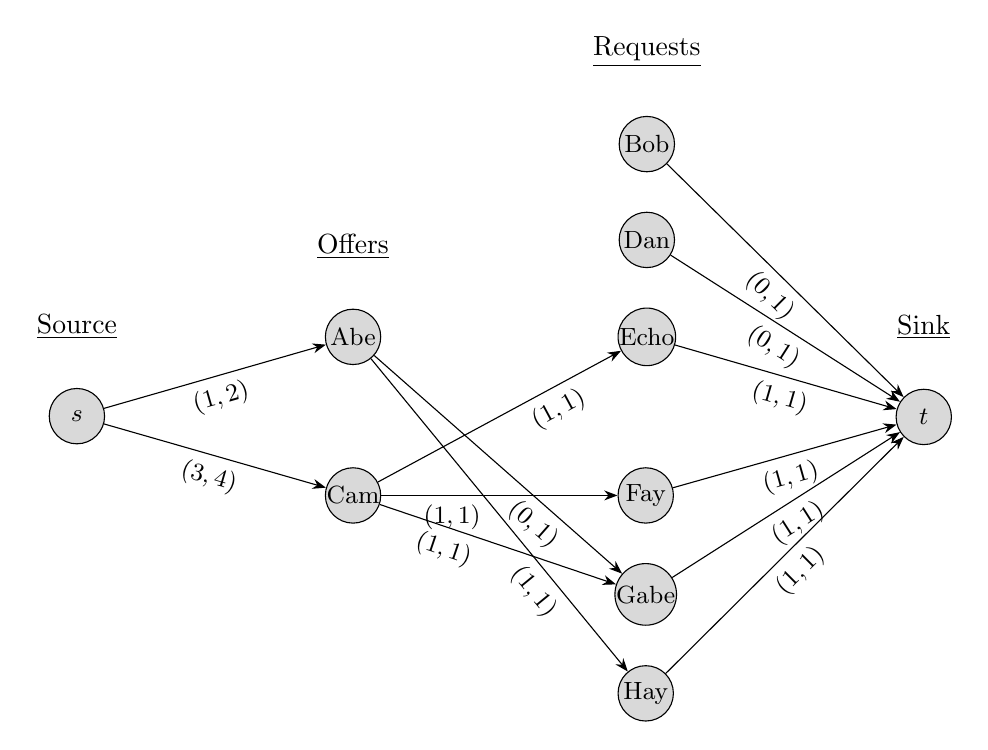
\begin{tikzpicture}[
      mycircle/.style={
         circle,
         draw=black,
         fill=gray,
         fill opacity = 0.3,
         text opacity=1,
         inner sep=0pt,
         minimum size=20pt,
         font=\small},
      myarrow/.style={-Stealth},
      node distance=0.5cm and 3cm
      ]
      \node[mycircle] (c1) {$s$};
      
      \node[mycircle,below right=of c1] (c2) {Cam};
      \node[mycircle,above right=of c1] (c4) {Abe};

      \node[mycircle,right=of c4] (c6) {Echo};
      \node[mycircle,right=of c2] (c7) {Fay};
      \node[mycircle,above=of c6] (c5) {Dan};
      \node[mycircle,above=of c5] (c3) {Bob};
      \node[mycircle,below=of c7] (c8) {Gabe};
      \node[mycircle,below=of c8] (c9) {Hay};
      
      \node[mycircle,below right=of c6] (c10) {$t$};

      % Titles above each stack of nodes
      \node[above=0.5cm of c1] {\underline{Source}};
      \node[above=0.5cm of c4] {\underline{Offers}};
      \node[above=0.5cm of c3] {\underline{Requests}};
      \node[above=0.5cm of c10] {\underline{Sink}};

    \foreach \i/\j/\txt/\p in {% start node/end node/text/position
      c1/c4/{$(1,2)$}/below,
      c1/c2/{$(3,4)$}/below,
      c6/c10/{$(1,1)$}/below,
      c7/c10/{$(1,1)$}/below,
      c5/c10/{$(0,1)$}/below,
      c3/c10/{$(0,1)$}/below,
      c8/c10/{$(1,1)$}/below,
      c9/c10/{$(1,1)$}/below}
       \draw [myarrow] (\i) -- node[sloped,font=\small,\p] {\txt} (\j);
    \foreach \i/\j/\txt/\p in {% start node/end node/text/position
      c4/c8/{$(0,1)$}/below,
      c4/c9/{$(1,1)$}/below,
      c2/c6/{$(1,1)$}/below}
       \draw [myarrow] (\i) -- node[sloped,pos=0.7,font=\small,\p] {\txt} (\j);
    \foreach \i/\j/\txt/\p in {% start node/end node/text/position
      c2/c7/{$(1,1)$}/below,
      c2/c8/{$(1,1)$}/below}
       \draw [myarrow] (\i) -- node[sloped,pos=0.3,font=\small,\p] {\txt} (\j);
    \end{tikzpicture}
    \end{center}
    Then, the evaluator finds the max flow values that can be send across these edges given their capacities via the Ford-Fulkerson/Edmonds-Karp algorithm. The maximal flow and residual graph (represented by the $flow$ value) is the maximal number of requests that can be satisfied by the existing offers. Each unit of flow pairs one offer with one request. The evaluator then recovers the residual graph and converts it to a nicely formatted output like this: \scriptsize
    \begin{verbatim}
MATCHED REQUESTS:
    Echo to Chicago at 10 PM on 5/22/2023 -> Cam to Chicago at 2 AM on 5/22/2023 to 10 AM on 5/23/2023
    Fay to Chicago at 10 PM on 5/22/2023 -> Cam to Chicago at 2 AM on 5/22/2023 to 10 AM on 5/23/2023
    Gabe to Arlington, Chicago at 5 PM on 1/1/2023 to 5 PM on 5/22/2023 -> Abe to Arlington at 2 PM on 1/5/2023 to 6 PM on 1/5/2023
    Hay to Arlington at 1 AM on 1/1/2023 to 11 PM on 1/9/2023 -> Abe to Arlington at 2 PM on 1/5/2023 to 6 PM on 1/5/2023

UNMATCHED REQUESTS:
    Bob to Boston at 5 PM on 1/3/2023
    Dan to Denver at 9 PM on 11/27/2023
    \end{verbatim} \normalsize
Which would be our final evaluation.

\subsubsection{The Benefits of Ford-Fulkerson/Edmonds-Karp}
A major benefit of reducing this problem to a flow network rather than iterating over offers and requests to find matches is that Ford-Fulkerson can undo matches it's made previously. Consider example program five.
\begin{verbatim}
Offer: Cam to Chicago at 2 AM on 1/5/2023 to 6 AM on 1/5/2023 with 2 seat
    Request: EchoOne to Chicago, Arlington at 2 AM on 1/5/2023
    Request: EchoTwo to Chicago, Arlington at 3 AM on 1/5/2023
    Request: EchoThree to Chicago at 4 AM on 1/5/2023
    Request: EchoFour to Chicago at 5 AM on 1/5/2023

Offer: Abe to Arlington at 2 AM on 1/5/2023 to 6 AM on 1/5/2023 with 5 seats
    Request: GabeOne to Arlington at 5 AM on 1/5/2023
    Request: GabeTwo to Arlington at 2 AM on 1/5/2023

Request: Bob to Boston at 5 AM on 1/5/2023
Request: Dan to Denver at 5 AM on 1/5/2023
\end{verbatim}
A naive solution may just match EchoOne and EchoTwo's request with Cam's offer since those appear first in the program and then put GabeOne and GabeTwo requests with Abe's offer. This leaves the remaining four requests EchoThree, EchoFour, Bob and Dan all unmatched. However, this is not the optimal solution. We could have done better by matching EchoThree and EchoFour with Cam and then EchoOne, EchoTwo, GabeOne, and GabeTwo with Abe, leaving the remaining 2 offers unmatched. The problem with the naive solution is that we can't undo a pairing we've made. Ford-Fulkerson, can undo a matching we've already made by sending flow backwards along a path, allowing us to undo a previous paring if we can make a better one. 

\newpage
\subsection{Remaining Work}
\begin{enumerate}
    \item In the last edition of the specification, we include BNF types to allow for an additional date format where months are written alphabetically instead of numerically. Thus, programs could include dates written like \verb|April 7, 2023| instead of \verb|4/7/2023|. We ended up not including this in the final implementation since we already allowed for one date format and wanted to focus our efforts on $Evaluator.fs$. Alternative date formats can be added to the parser and would not change any of the underlying AST types.

    \item It's common for people asking for rides to offer snacks, gas money, or compensation. As we demonstrated with the other input fields in this PL, one could add a compensation field to offers/requests. For example maybe $Jacob$'s offer should only be paired with requests that pay for gas in the evaluated result. Given more time we'd like to add an option field for this in the PL.

    \item F\#'s built-in $DateTime.TryParse$ function is very forgiving. If it can parse but not interpret the date which we have given it defaults to \verb|12 AM on 1/1/0001|. For example, if we were to write the following date as input to our program: 
    \begin{center}
        at 65 PM on 9999/9999/9999
    \end{center}
    Then the following is the date that $DateTime.TryParse$ would return after parsing that line:
    \begin{center}
        at 12 AM on 1/1/0001
    \end{center}
    This means that given a crazy date, the program will still run, but will be incorrect, as offers may be matched to 12AM on 1/1/0001 which should not be matched at all. Therefore, as a future improvement, we would want to place more restrictions on what dates can be inputted, so that the F\# $DateTime.TryParse$ does not return any odd dates.



\end{enumerate}



% DO NOT DELETE ANYTHING BELOW THIS LINE
\end{document}
Powered by Gitea Licenses APIhttps://www.overleaf.com/project/6559206e9c96f59e4ca20601